%%%%%%%%%%%%%%%%%%%%%%%%%%%%%%%%%%%%%%%%%%%%%%%%%%%%%%%%%%%%%%%%%%%%%%%%%%%%%%%%%%%%%%%%
%
%   Context of the Project
%
%%
%%%%%%%%%%%%%%%%%%%%%%%%%%%%%%%%%%%%%%%%%%%%%%%%%%%%%%%%%%%%%%%%%%%%%%%%%%%%%%%%%%%%%%
\section{Introduction}

\subsection{Context}

Today mastering his domestic energy consumption is a major stake in our society. Everyear, bills related to energetic ressources increase, in 2013 French homes paid 3210\euro, an increase of more than 40\euro\ compared with 2012. And the ways set up to reduce them such as solar panels are still too expensive for the majority of the population and not enough effective during winter seasons.\\

%ref pour les 3210\euro : page 31 http://www.statistiques.developpement-durable.gouv.fr/fileadmin/documents/Produits_editoriaux/Publications/References/2014/references-bilan-energie2013-ed-2014-t.pdf

In this context, the global objective of the project is to work on the design of a "box" called Smartee that can minimize the energy consumption of a building and maximize comfort. The Smart-Eco Box project was developed in a new growing market, known as Smart Energy Boxes. Although many sensors are already on the market, they are usually heterogeneous (i.e. non-standardized ) which complicates their use in a system such as the one we would like to develop. Therefore members of the project will design a wireless communication system (box + associated sensors) for intelligent and efficient supervised management of energy consumption of a building on a website including the ability of the box to identify an electrical device in its ignition.\\

%Dans un monde de plus en plus connecté et soucieux de l’environnement, nos maisons se transforment en habitats intelligents, et permettent notamment une meilleure gestion des dépenses énergétiques au quotidien. Ces dernières années, de nombreux systèmes de domotique assurant la gestion des équipements (portails, volets, lumières) sont arrivés sur le marché. Néanmoins, très peu de ces systèmes permettent le suivi détaillé et le pilotage énergétique de l’ensemble des équipements au sein de l’habitat. Période de crise et diminution du pouvoir d’achat poussent les Français à réaliser des économies dans tous les domaines. Selon l’ADEME (Agence de l’environnement et de la maîtrise de l’énergie), la facture moyenne (toutes énergies confondues) s’est élevée en 2012 à 1 403 euros par ménage, contre 1 239 euros en 2007. Aujourd’hui, 80\% des ménages cherchent à réduire leur consommation d’énergie, notamment via des comportements plus économes en terme d’éclairage et de chauffage. Un nouveau secteur est en train de naître, les smart energy boxes. Certains fabricants du domaine énergétique tels que Legrand ou Schneider Electric proposent déjà des solutions comme les premiers compteurs électriques connectés. Le projet Ecobox s’inscrit dans une démarche de meilleure gestion de l’énergie par un pilotage autonome et automatisée de l’habitat.

\subsection{Smart EcoBox Description}
% Quel est le but de la box ?
%
% déroulement du process : recevoir trame, décoder, inserer dans db. detection des états des appareils. affichage des infos sur le client.
%
% pourquoi avoir choisi Raspberry Pi ?
%   box doit être petite (cad pas un gros pc etc..)
%   peu cher -> correspond au souhait du client d'avoir une box abordable
%   comme ça a peu de ressources, si ça passe dessus peu importe les ressources dispo dans le future


The \textbf{Smart EcoBox} project is aimed toward helping people control their energy consumption and therefore reduce their energy bills. With this system, the user is able to foresee and handle what he consumes through his mobile device with the help of sensors he set up in his home. The main computer processing is gathered in a small and cheap computer called Raspberry Pi to respect the client's needs.

%La gestion des équipements de la maison par l’intermédiaire de terminaux tels que tablettes ou téléphones permettra de simplifier la vie de l’utilisateur au quotidien.

\begin{figure}[H]
\centering
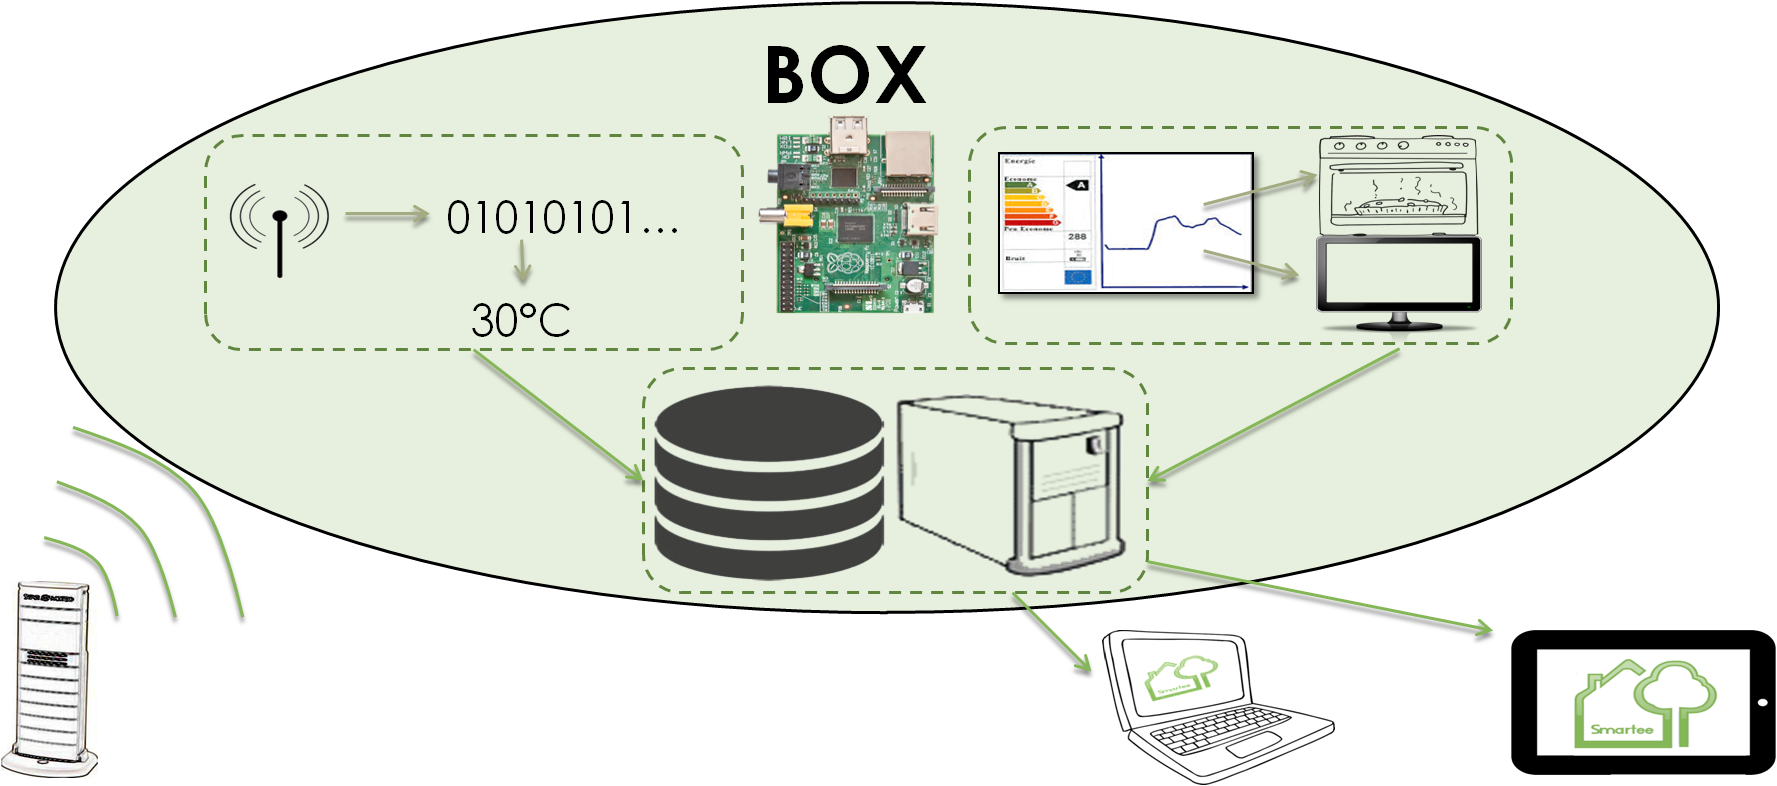
\includegraphics[scale=0.5]{figures/box.png}
\caption{Smart Eco Box Description}
\label{fig:boxDescription}
\end{figure}

As seen in the figure \ref{fig:boxDescription}, the Raspberry Pi called "BOX" gathers the main algorithms that interact with the data received from the sensors. Firstly, the box detect the data send by the sensors detected in the home. An algorithm decode those data and store them in a database. Meanwhile, an other algorithm detect which device is turned on or not using the previous data and store those information in the database. A web application enable the user to manage those information, in other words his energy consumption.

%Once plugged in, the Smartee initialization detects sensors in the environment. Then a processing phase allows the box to work without any need for input by the client. This software allowed to detect bursts and initiated bursts processing received by a provided Universal Software Radio Peripheral (USRP). Finally data are stored in a database. The place's energy consumption is displayed on the website.
